\chapter{Data Preparation}  \label{chapter:data-preparation}
As it is often the case with data science projects, the data preparation part takes time and effort. After the static and time series bond data has been extracted from Datastream -- which will likely take several days -- it is available in form of multiple data parts in Excel format. Since it is more convenient to perform further statistical analysis in a dedicated statistical environment, such as Stata or MatLab, the data needs to be brought into 'long' format, and additionally to be cleaned from null entries and outliers. The undertaken procedures are described in the following. 

\section{Data Formatting}  \label{section:data-formatting}
For the static bond data, there is not much to be done in terms of formatting. Its original format, as downloaded from Datastream, is mostly suitable for further analysis and can be directly imported into Stata. 

The downloaded time series data is initially in 'wide' format and has multiple bonds in one row. It looks like shown in Fig. \ref{fig:original-excel-ts-data}. 

\begin{figure}[h]
	\centering
	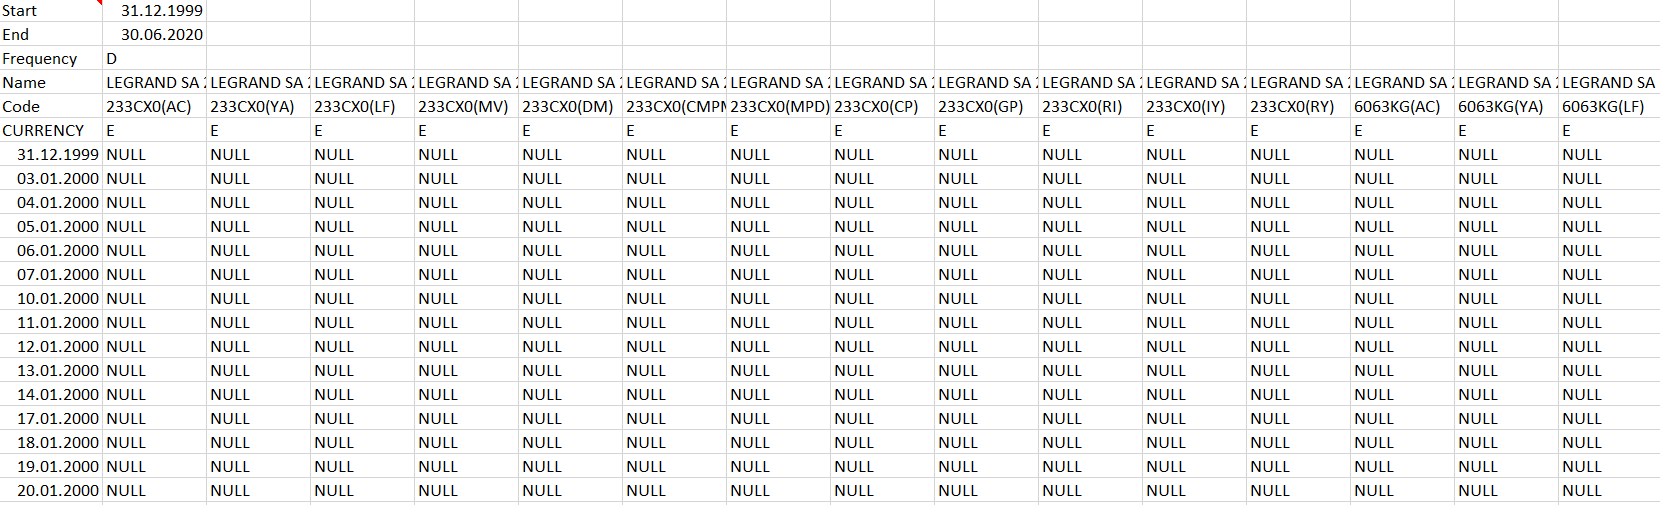
\includegraphics[width=1.0\linewidth]{figures/original-excel-ts-data}
	\caption{Sample of downloaded raw time series bond data}
	\label{fig:original-excel-ts-data}
\end{figure}

The goal is to transform this time series data into 'long' format, as can be seen in Fig. \ref{fig:long-format-excel-ts-data}, by saving the bonds one below the other. 
\begin{figure}[h]
	\centering
	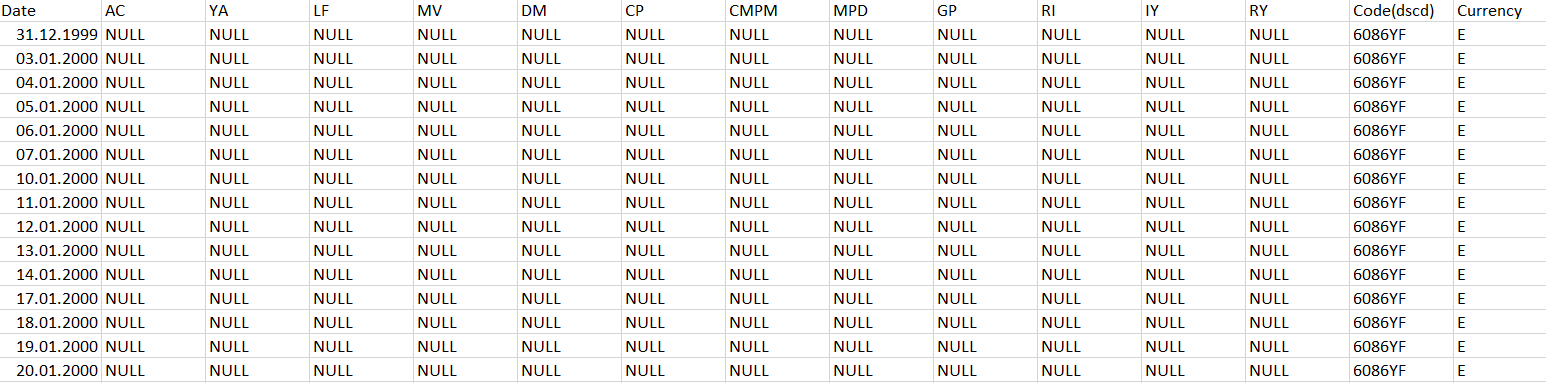
\includegraphics[width=1.0\linewidth]{figures/long-format-excel-ts-data}
	\caption{Sample of downloaded time series bond data in 'long' format}
	\label{fig:long-format-excel-ts-data}
\end{figure}
Additionally, the header has to be removed, and the \textit{dscd} identifier of each bond as well as its currency have to be entered as a separate column for each date instead of being at the top. 

I wrote a VBA macro with a function called \textit{ToLongFormat} (which can be found in project files) which accomplishes the described task. While Stata might have also been able to do the formatting, I decided to work with VBA at this point, since it is native to the MS Excel environment. The main procedure is as follows: 
\begin{enumerate}
	\item Define data layout constants depending on the initial format: header height, number of time stamps, number of datatypes, bonds per block, and number of blocks. A block is defined as all time stamps for multiple bonds which are located row-wise next to each other. An example can be seen in Fig. \ref{fig:original-excel-ts-data} where two bonds from the same firm, but with different \textit{dscd} codes, are next to each other. There can be multiple such blocks one below the other in one Excel file, depending on how the data was downloaded. 
	\item For all data files (as there will be multiple for larger requests) and for all blocks within each file, remove the header rows, place bonds one below the other, and create columns for \textit{dscd} and currency. 
	\item Add a newly created header row once at the beginning of the file. This header row can later be used to define variable names in statistical software. 
\end{enumerate}

Note that if the original Excel files are very large, i.e. with a high amount of securities or dates, Excel might reach its sheet length limit when running this macro. If you notice such behavior, there is another function shipped with this macro, called \textit{SplitInSubfiles()}. You can use this function on your initial downloaded Excel data to reshape it into smaller-sized files, before transforming it to 'long' format. 

\section{Stata Import} \label{section:data-cleaning}
As soon as the data has been formatted, it can be cleaned conveniently within statistical software. Since I am working with Stata, the Excel files with static as well as reshaped time series data can be simply imported to Stata with the \textit{import excel} Stata command. It is possible to save frequently used Stata scripts in form of \textit{.do} files to reuse them later. You can find all the do-files involved in this project in the respective folders for this project step. 

The static bond data merely needs to be checked for duplicates, e.g. by using the \textit{duplicates report} Stata command. Empirically, static data extracted from Datastream is significantly cleaner than historical pricing data. 
Therefore, all the following cleaning procedures only need to be applied to the time series data.

Because Stata can generally work with larger files than Excel, it makes sense to merge the imported time series files -- now already in Stata format -- to files of larger size, which will make further work more convenient. After the data has been imported to Stata, it can now be cleaned with the help of standard Stata procedures.  

\section{Data Cleaning}
For cleaning, multiple different procedures need to be applied. Since they are all commutative, it does not make a difference in which order these are executed. 
\begin{itemize}
	\item Null values can be cleaned with the \textit{drop} command, e.g. with \\ \lstinline{drop if MPD=="NULL" | MPD==""}. 
	Be prepared for a lot of values to be deleted when working with historical bond data. This is due to many bonds having been issued recently and thus not having older price entries. 
	\item Erroneous values which sometimes occur in Datastream typically have high length. Remove these with e.g. \lstinline{drop if length(var) > 40}, with \textit{var} being the variable names. 
	\item Cast date stamps from string to date format. This can be done by generating a new variable for the date first (\lstinline{gen date = date(Date, "MDY")}). Then the new variable should be formatted to be well-readable (format date \%tdnn/dd/CCYY). After that the old variable \textit{Date} can be dropped, so that the newly created \textit{date} takes its place. 
	\item Cast integer and double values that are coded as strings back to numeric, e.g. with the \lstinline{destring} command. 
	\item Remove duplicates based on the variables \textit{date} and \textit{dscd}. There should not be two or more different entries for the same security on the same date.
\end{itemize}
Keep in mind to manually check the resulting data. No matter how thorough the cleaning procedure, there might still be some erroneous data which needs to be cleaned up or removed manually. Besides the listed cleaning methods, the data should additionally be searched for outliers that can have a negative impact on the further analysis. However, different values and tuples can be considered outliers depending on the analysis scenario. Therefore, I decided to leave the (not necessarily erroneous) outliers in the dataset at this step of the project. They will be filtered out as shown in chapter \ref{chapter:statistical-analysis} later on. 

After the data has been cleaned, many tuples will have been deleted. To make further analysis more convenient, it therefore makes sense to merge all the single data files into one. While it depends on the size of the entire dataset, this should still be possible in most cases. Otherwise, e.g. two or three files can be produced in total. Files can be merged easily in Stata, e.g. by using the \lstinline{append} command. Having done that, the resulting cleaned and compact data is now ready for future statistical analysis. 